\documentclass{article}
\usepackage{tikz}

\begin{document}

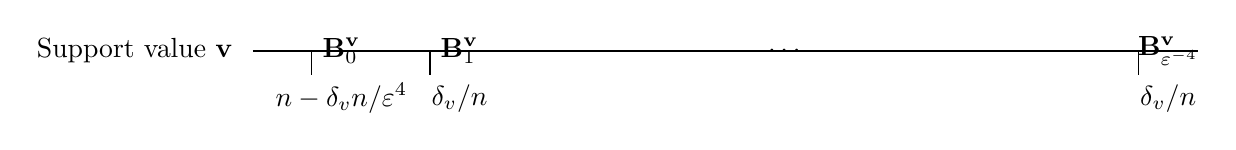
\begin{tikzpicture}[scale=1.5]
    % Draw the horizontal line
    \draw (0,0) -- (8,0);
    
    % Draw the vertical lines
    \draw (0.5,0) -- (0.5,-0.2);
    \draw (1.5,0) -- (1.5,-0.2);
    \draw (7.5,0) -- (7.5,-0.2);
    
    % Label the sections
    \node at (0.75,0) {$\mathbf{B}_{0}^{\mathbf{v}}$};
    \node at (1.75,0) {$\mathbf{B}_{1}^{\mathbf{v}}$};
    \node at (7.75,0) {$\mathbf{B}_{\varepsilon^{-4}}^{\mathbf{v}}$};
    
    % Draw the ellipsis
    \node at (4.5,0) {$\cdots$};
    
    % Draw the labels below each section
    \node at (0.75,-0.4) {$n - \delta_{v} n / \varepsilon^{4}$};
    \node at (1.75,-0.4) {$\delta_{v} / n$};
    \node at (7.75,-0.4) {$\delta_{v} / n$};
    
    % Draw the support value label
    \node at (-1,0) {Support value $\mathbf{v}$};
\end{tikzpicture}

\end{document}